\documentclass[../CSC_5RO07_TA.tex]{subfiles}

\begin{document}
\section{Q3: Multicoeur 5 coeurs : 1 ARM et 4 MicroBlaze}

\subsection{Flux de travail}

Comme précédemment, le flux de traitement du système est décrit (Figure \ref{fig:8}), cependant dans ce scénario, un système à 5 cœurs est utilisé avec un processeur ARM 9 et 4 processeurs Microblaze.

\begin{figure}[H]
    \centering
    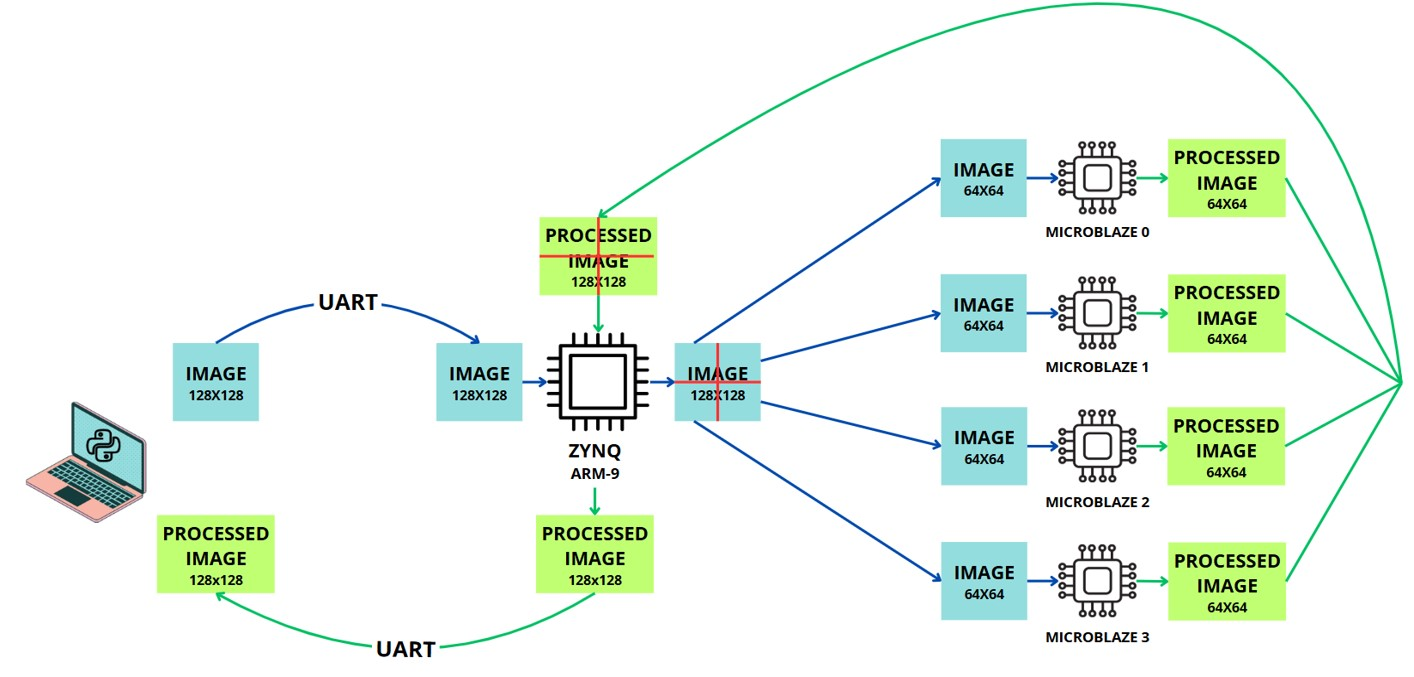
\includegraphics[width=0.8\columnwidth]{./images/DiagramaBloques5x5.jpg}
    \caption{Schéma explicatif du flux de travail du système.}
    \label{fig:8}
\end{figure}

L'envoi de l'image entre l'ordinateur et l'ARM est le même que précédemment, en utilisant l'interface UART.

\vspace{1em} 

De la même manière, lors de la réception de l'image complète, l'ARM 9 la divise en quatre sous-images de dimensions égales. Cependant, cette fois la répartition des sous-images se fait en tenant compte des deux nouveaux processeurs.

\begin{itemize}
    \item MicroBlaze 0 : Traite la sous-image correspondant au premier quart de l'image, située dans le coin supérieur gauche.
    \item MicroBlaze 1 : Responsable de la sous-image correspondant au deuxième quart de l'image, située dans le coin supérieur droit.
    \item MicroBlaze 2 : Traite la sous-image correspondant au troisième quart de l'image, situé dans le coin inférieur gauche.
    \item MicroBlaze 3 : Il est responsable de la sous-image correspondant au quatrième et dernier quart de l'image, située dans le coin inférieur droit.
\end{itemize}

Les étapes restantes du processus sont effectuées de manière identique à ce qui a été décrit pour le système à 3 processeurs décrit ci-dessus.

\subsection{Diagramme de blocs}

\begin{figure}[H]
    \centering
    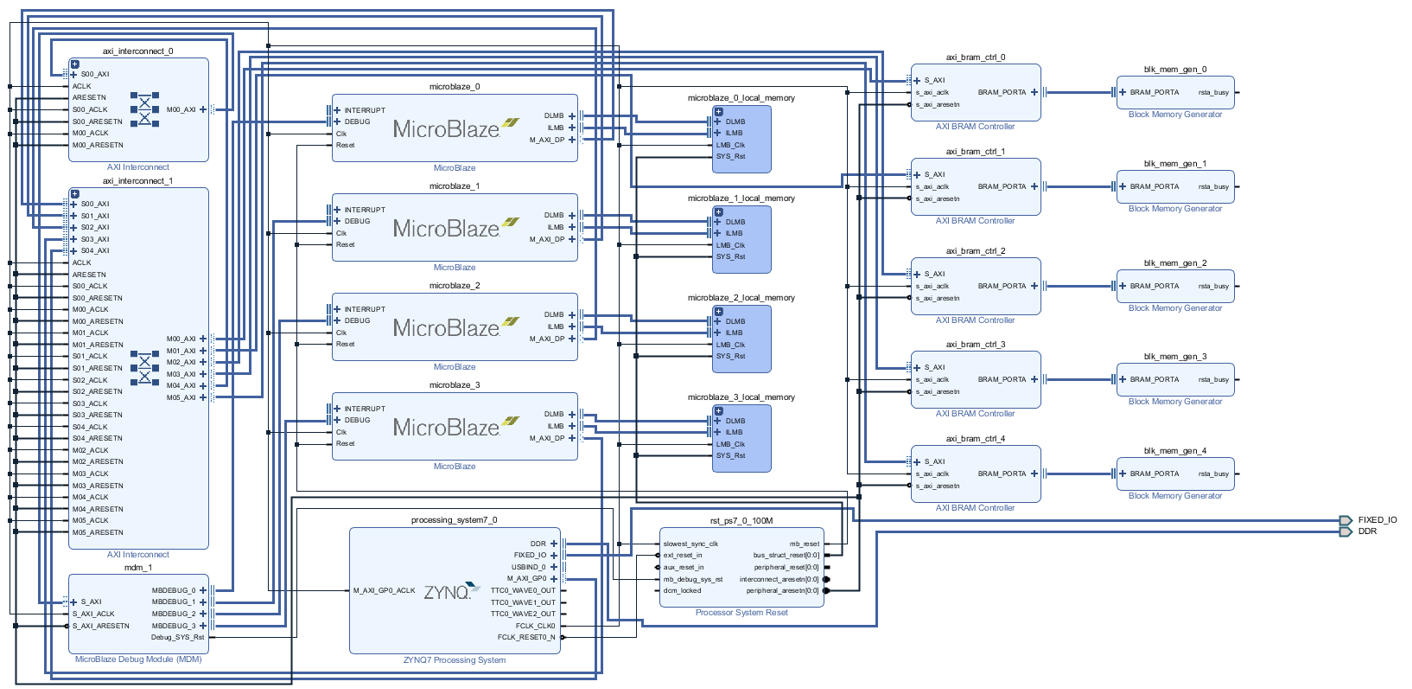
\includegraphics[width=1.0\columnwidth]{img3}
    \caption{Répartition de la mémoire.}
    \label{fig:9}
\end{figure}

Le système est conçu avec un \textbf{ZYNQ7 Processing System} et \textbf{quatre processeurs MicroBlaze} pour les tâches de traitement d'images. Le ZYNQ7, avec ses deux cœurs ARM Cortex-A9, agit comme l'unité centrale, gérant les tâches générales, la communication avec les périphériques, et le transfert de données vers la mémoire DDR et les blocs logiques programmables. 

\subsubsection{Processeurs MicroBlaze}  
Le système inclut désormais \textbf{quatre processeurs MicroBlaze}, chacun étant affecté à une partie spécifique du traitement d'image. Ces processeurs fonctionnent en parallèle, ce qui améliore considérablement les performances du système. Chaque MicroBlaze est responsable du traitement d'une section distincte de l'image, en appliquant le filtre Sobel pour détecter les contours. Ce traitement parallèle permet au système de gérer des volumes de données plus importants et d'accélérer le traitement des images.

\subsubsection{Mémoire Locale pour les Processeurs MicroBlaze}  
Pour assurer un traitement rapide et efficace, chaque processeur MicroBlaze dispose de sa propre \textbf{mémoire locale}, spécifiquement le \textbf{DLMB} (Data Local Memory) et le \textbf{ILMB} (Instruction Local Memory). Cela permet à chaque MicroBlaze de fonctionner de manière autonome, avec un accès rapide aux données et instructions nécessaires pour le traitement en temps réel. L'ajout de deux mémoires locales supplémentaires fournit davantage de ressources dédiées pour les nouveaux processeurs MicroBlaze, permettant ainsi une optimisation et une parallélisation plus poussées de la charge de travail.

\subsubsection{BRAM et Contrôleurs}  
Le système utilise des \textbf{Block RAMs (BRAMs)}, gérées par les \textbf{AXI BRAM Controllers}, pour stocker les fragments d'image et les résultats intermédiaires pendant le processus de détection des bords. Avec l'ajout de \textbf{trois contrôleurs BRAM supplémentaires} et \textbf{blocs de mémoire BRAM}, le système a augmenté sa capacité de stockage temporaire. Ces nouvelles BRAMs agissent comme des tampons pour chaque processeur MicroBlaze, réduisant la latence et garantissant un débit élevé pendant le traitement de grandes quantités de données d'image. La structure BRAM élargie permet aux processeurs de stocker davantage de données intermédiaires localement, accélérant ainsi le processus global.

\subsubsection{AXI Interconnects}  
Les \textbf{AXI Interconnects} servent de colonne vertébrale pour la communication, facilitant les transferts de données entre le ZYNQ7, les processeurs MicroBlaze, les mémoires locales, les contrôleurs BRAM et les autres périphériques. Avec l'ajout de plus de BRAM et de processeurs MicroBlaze, les interconnexions sont cruciales pour gérer l'augmentation du flux de données. Elles garantissent que chaque composant reçoive rapidement et efficacement les données dont il a besoin, soutenant le débit élevé nécessaire pour le traitement d'images en temps réel.

\subsubsection{Débogage des MicroBlaze et Réinitialisation du Système}  
Le \textbf{MicroBlaze Debug Module} permet la surveillance et le débogage en temps réel des processeurs MicroBlaze, garantissant que toutes les tâches de traitement sont effectuées correctement. La \textbf{réinitialisation du système processeur} assure que le système démarre de manière synchronisée, évitant tout problème d'initialisation et maintenant la stabilité du design.

\subsubsection{Vue d'Ensemble du Système}  
En résumé, le design exploite la puissance du ZYNQ7 pour le traitement général, la flexibilité des quatre processeurs MicroBlaze pour les tâches spécifiques de traitement d'images, la capacité améliorée des mémoires locales et des BRAM pour un traitement efficace des données, et les interconnexions AXI pour un flux de données fluide entre tous les composants. Ce système étendu est capable de gérer des tâches de traitement d'images plus complexes, avec une parallélisation et une efficacité accrues, ce qui en fait une solution idéale pour des applications en temps réel où la rapidité et la capacité à traiter de grands volumes de données sont cruciales.

\subsection{Mémoires}

De la même manière que précédemment, le système implémente une structure de mémoire hiérarchique conçue pour optimiser l'interaction entre quatre processeurs MicroBlaze et un système Zynq basé sur un ARM Cortex-A9. Ce schéma organise et segmente la mémoire pour diviser efficacement la charge de travail entre différents éléments, facilitant ainsi le traitement parallèle et une gestion efficace des ressources.

\vspace{1em}

Par rapport au cas précédent, deux mémoires locales ont été ajoutées pour chaque microblaze et deux mémoires partagées supplémentaires, qui permettent la coordination entre les MicroBlaze et facilitent le transfert de données entre les différents processeurs.

\vspace{1em}

La taille de la mémoire est restée à 32 Ko et deux nouveaux espaces mémoire ont été ajoutés (0x44000000 - 0x44007fff et 0x46000000 - 0x46007fff). La nouvelle distribution peut être revue dans la figure \ref{}.

\begin{figure}[H]
    \centering
    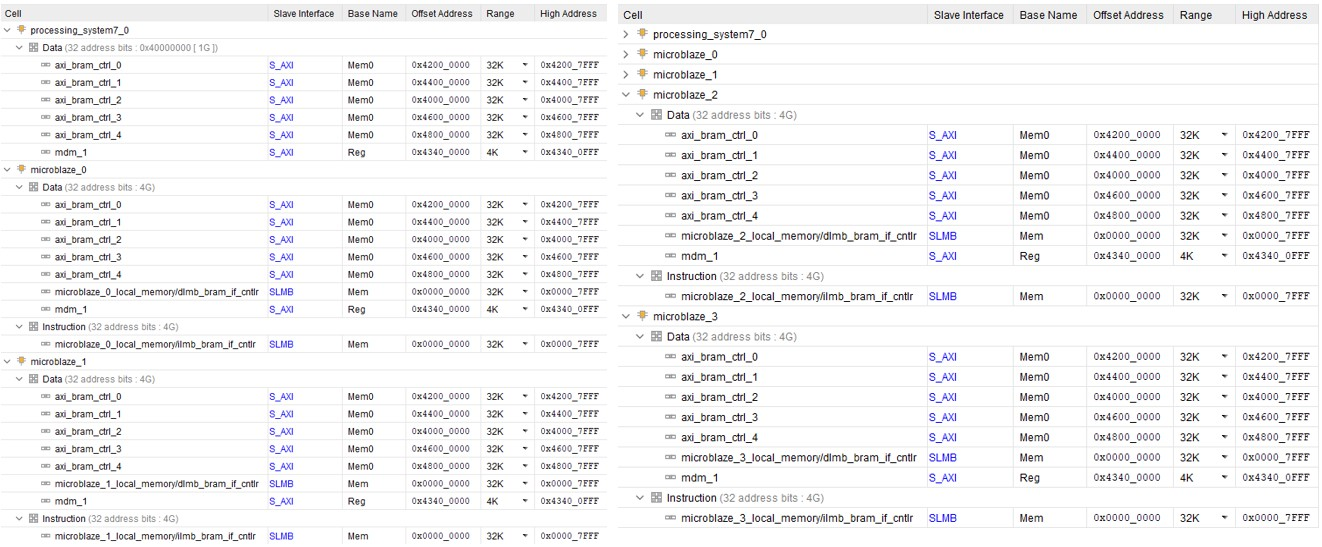
\includegraphics[width=1.0\columnwidth]{./images/Memoria2.jpg}
    \caption{Répartition de la mémoire.}
    \label{fig:010}
\end{figure}

De plus, le système de paralysie proposé précédemment a été maintenu, avec écrasement des masques ($G_x$ et $G_y$).


\subsection{Résultats}


\subsubsection{Temps de traitement}

Le temps nécessaire au système pour traiter les images par les quatre Microblazes, après que chaque quart d'entre elles soit placé dans la mémoire partagée, est de 13 ms. 

Si l'on compare cela avec le résultat obtenu précédemment (27 ms), on constate que c'est la moitié du temps précédent. Ce résultat est conforme à ce que l'on attend de ce système, puisqu'il dispose de deux fois plus de processeurs en charge du traitement de l'image, ce qui parallélise complètement la tâche et réduit donc cette valeur.

\begin{figure}[H]
    \centering
    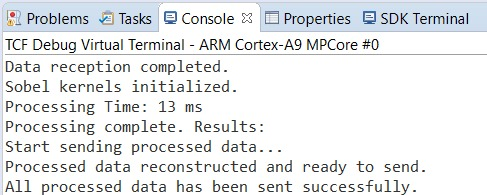
\includegraphics[width=0.5\columnwidth]{./images/Resutlado2.jpg}
    \caption{Temps de traitement des images.}
    \label{fig:11}
\end{figure}
\end{document}
